%!TEX TS-program = xelatex
\documentclass{beamer}

\usepackage{HSE-theme/beamerthemeHSE} % Подгружаем тему

%%% Работа с русским языком и шрифтами
\usepackage[english,russian]{babel}   % загружает пакет многоязыковой вёрстки
\usepackage{fontspec}      % подготавливает загрузку шрифтов Open Type, True Type и др.
\defaultfontfeatures{Ligatures={TeX},Renderer=Basic}  % свойства шрифтов по умолчанию

\usepackage{xltabular}
\usepackage{calc}
\usepackage{adjustbox}
\usepackage{lipsum}
\usepackage{microtype}
\usepackage{vwcol}  
\usepackage{subfig}
\usepackage[fleqn]{mathtools}
\usepackage{listings}
\lstset{language=C++,
                basicstyle=\ttfamily,
                keywordstyle=\color{blue}\ttfamily,
                stringstyle=\color{red}\ttfamily,
                commentstyle=\color{green}\ttfamily,
                morecomment=[l][\color{magenta}]{\#}
}

% \usepackage{graphicx}


\setmainfont[
Path = fonts/,
BoldFont = MyriadPro-Bold.otf,
ItalicFont = MyriadPro-It.otf,
BoldItalicFont = MyriadPro-BoldIt.otf]
{MyriadPro-Regular.otf}

% \usetheme{Madrid}
% \usecolortheme{beaver}

\setsansfont[
Path = fonts/,
BoldFont = MyriadPro-Bold.otf,
ItalicFont = MyriadPro-It.otf,
BoldItalicFont  = MyriadPro-BoldIt.otf]
{MyriadPro-Regular.otf}

\newcounter{nameOfYourChoice}






% \setmainfont[Ligatures={TeX,Historic}]{Arial} %  установите шрифты Myriad Pro или (при невозможности) замените здесь на другой шрифт, который есть в системе — например, Arial

% \setsansfont{Arial}  %  установите шрифты Myriad Pro или (при невозможности) замените здесь на другой шрифт, который есть в системе — например, Arial
\setmonofont{Courier New}
\uselanguage{russian}
\languagepath{russian}
\deftranslation[to=russian]{Theorem}{Теорема}
\deftranslation[to=russian]{Definition}{Определение}
\deftranslation[to=russian]{Definitions}{Определения}
\deftranslation[to=russian]{Corollary}{Следствие}
\deftranslation[to=russian]{Fact}{Факт}
\deftranslation[to=russian]{Example}{Пример}
\deftranslation[to=russian]{Examples}{Примеры}

\usepackage{multicol}         % Несколько колонок
\graphicspath{{images/}}      % Папка с картинками

%%% Информация об авторе и выступлении
\title[Заголовок]{Факультет компьютерных наук, 
Образовательная программа <<Прикладная математика и информатика>>\\
Программный проект
} 
\subtitle{<<Подготовка задач для олимпиад школьников>>}
% \author[Деб Натх М., БПМИ181]{Деб Натх Максим \\ \smallskip \scriptsize \url{author@hse.ru}\\\url{http://hse.ru/staff/author/}}
\author[Деб Натх М., БПМИ181]{Выполнил Деб Натх Максим, БПМИ181\\{\small Руководитель:
Густокашин Михаил Сергеевич, директор Центра студенческих олимпиад, ФКН
ВШЭ }}

\institute[\tiny{<<Подготовка задач для олимпиад>>}]{}
\date{29 июня 2020 г.}

\begin{document}    % Начало презентации

\frame[plain]{\titlepage}    % Титульный слайд






\begin{frame}
\frametitle{Описание предметной области}
Предметная область проекта~--- разработка задач для соревнований по программированию, в том числе состязаний для школьников по программированию, проводимых НИУ ВШЭ, а именно, <<Высшая проба по информатике>>, <<Московская олимпиада школьников по информатике>> .

\end{frame}








\begin{frame}
\frametitle{Основные понятия, определения, термины}
\begin{itemize}
 \item<1-> \emph{Задача по олимпиадному программированию}~--- проблема, для решения которой необходимо придумать и реализовать алгоритм. Задача считается решённой, если участник смогли составить программу, правильно работающую на тестовых примерах, подготовленных жюри.
 \item<2-> \emph{Проверяющая программа (checker)}~--- программа, сверяющая вывод на конкретном тестовом примере ответ участника и ответ жюри и возвращающая вердикт по данному тестовому примеру.
 \item<3-> \emph{Валидатор (validator)}~--- программа, проверяющая корректность входных данных.
 \item<4-> \emph{Генератор (generator)}~--- программа, генерирующя тестовые примеры.
\end{itemize}
\end{frame}








\begin{frame}
\frametitle{Актуальность работы}
Ежегодно в России проходит несколько десятков перечневых олимпиад по программированию, для их проведения которых необходим набор оригинальных задач. Задачи эти должны затрагивать различные области математики, компьютерных наук, алгоритмов и структур данных. 
\bigskip

\emph{ <<Высшая проба по информатике>> } и \emph{ <<Московская олимпиада школьников по программированию>> } входят в число таких олимпиад. Они проводятся при поддержке центра студенческих олимпиад ФКН.
\end{frame}








\begin{frame}
\frametitle{Цель и задачи работы}
Целью проекта была подготовка пакета нескольких задач по спортивному программированию, которые будет возможно использовать вместе с системами \emph{ejudge} или \emph{Яндекс.Контест}.

\bigskip
Задачи:
\begin{enumerate}
\item<1-> Разработка задачи, её анализ, разработка её решения
\item<2-> Реализация решения задачи на одном из поддерживаемых языков программирования
\item<3-> Реализация вспомогательных программ~--- валидатора, чекера, генераторов
\item<4-> Создание группы тестов для проверки решений
\end{enumerate}
\end{frame}








\begin{frame}
\frametitle{Анализ существующих решений}
    \fontsize{12pt}{7.2}\selectfont

В силу технологических особенностей олимпиада <<Высшая проба>> проводится на платформе \emph{ejudge}\footnote{\url{https://ejudge.ru}}, <<Московская олимпиада школьников>> проводится на платформе \emph{Yandex.Contest}\footnote{\url{https://contest.yandex.ru}}. 

\bigskip
В связи с этим задачи необходимо будет готовить в формате пакетов, поддерживаемых этими системами. 

\bigskip
\emph{ <<Codeforces Polygon>> }\footnote{\url{https://polygon.codeforces.com}}~--- единственная крупная и наиболее популярная система подготовки задач, её формат является де-факто стандартом в подготовке задач. Поддерживает экспортирование на платформы Yandex.Contest и ejudge.
\end{frame}








\begin{frame}
\frametitle{Функциональные и нефункциональные требования}
\begin{enumerate}
\item Работоспособность при использовании тестирующей системой подготовленного пакета задач.
\item Возможность отправить произвольное решение в систему и получить вердикт по нему (\texttt{OK}, \texttt{WA}, \texttt{PE}, \texttt{TL}, \texttt{ML}, \texttt{CE}).
\item Корректная работа тестирующей программы на правильных и неправильных решениях.
\setcounter{nameOfYourChoice}{\value{enumi}}
\end{enumerate}
Описанные выше требования продиктованы функциональными особенностями систем и общепринятыми стандартами.
\begin{enumerate}
    \setcounter{enumi}{\value{nameOfYourChoice}}
    \item Требование в решении задачи знаний в использовании алгоритмов и структур данных, умения пользоваться языками программирования.
    \item Нетривиальность решения.
\end{enumerate}
\end{frame}








\begin{frame}
\frametitle{Задача №1}
    Задача была предложена на втором отборочном этапе олимпиады <<Высшая проба>>. Этот этап проходил в качестве онлайн-тура длительностью 3 часа на платформе ejudge. 
\end{frame}








\begin{frame}
\frametitle{Задача №1}
\framesubtitle{Условие}

\begin{columns}[onlytextwidth]
\begin{column}{0.3\textwidth}
    \begin{figure}
    \centering
    \caption{$N = 3$, $K = 2$}
    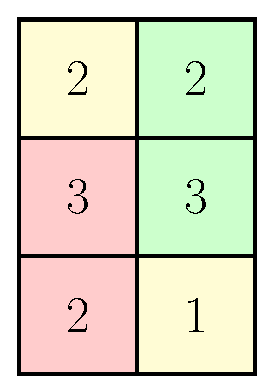
\includegraphics[width=0.9\textwidth]{drawing-1/drawing-figure0.eps}
    \end{figure}
\end{column}

\begin{column}{0.7\textwidth}
    \begin{itemize}
        \item Дана полоска (матрица) натуральных чисел размера $2 \times N$ и натуральное число $K$.
        \item Требуется разместить на данной полоске ровно $K$ непересекающихся костей домино (матриц $2\times1$ или $1\times 2$) таким образом, чтобы сумма чисел на непокрытых костями клетках была минимальна. 
        \item Требуется найти восстановить любую конфигурацию, на которой достигается этот минимум.
    \end{itemize}
\end{column}
\end{columns}
\end{frame}








\begin{frame}
\frametitle{Задача №1}
\framesubtitle{Условие}

\begin{multicols}{2}
\emph{Ограничения тестов:}
\begin{itemize}
    \item $1 \leqslant N \leqslant 2 \cdot 10^{5}$;
    \item $0 \leqslant K \leqslant 2 \cdot 10^{5}$;
    \item $0 \leqslant N \times K \leqslant 2 \cdot 10^{5}$;
    \item $K \leqslant N$;
\end{itemize}
\columnbreak
\emph{Ограничения на решение задачи:}
\begin{itemize}
    \item Ограничение по виртуальной памяти: 256MB
    \item Ограничение по виртуальному времени: 1 сек.
\end{itemize}

\end{multicols} 

\end{frame}








\begin{frame}
\frametitle{Задача №1}
\framesubtitle{Решение}
\fontsize{11pt}{7.2}\selectfont

\begin{itemize}
\item Заметим, что задача минимизации суммы непокрытых клеток равносильна задаче максимизации суммы покрытых клеток.

\item Воспользуемся методом многомерного динамического программирования.

\item Обозначим за \texttt{dp[k][i][j]}, где $0 \leq i \leq N$, $0 \leq j \leq K$, $0 \leq k \leq 3$  максимальную сумму покрытых клеток, если рассматривается задача покрытия первых $i$ столбцов $j$ костями, при этом в последнем ряду:

\[
\begin{array}{ll}
        \text{ни одна клетка не покрыта} &\text{, если $k = 0$;}\\
        \text{только первая клетка покрыта} &\text{, если $k = 1$;}\\
        \text{только вторая клетка покрыта} &\text{, если $k = 2$;}\\
        \text{обе клетки покрыты} &\text{, если $k = 3$;}\\
\end{array}
\]

\item В таком случае максимальная сумма будет равна  $\max\limits_{0 \leq k \leq 3}$\texttt{dp[k][N][K]}.

\end{itemize}
\end{frame}








\begin{frame}
\frametitle{Задача №1}
\framesubtitle{Решение}
\fontsize{10pt}{7.2}\selectfont
\begin{itemize}
\item По определению \texttt{dp} имеем, что 
$$\text{\texttt{dp[0][i][j]} = $\max\limits_{k}$ \texttt{dp[k][i-1][j]}}$$

\end{itemize}
\end{frame}








\begin{frame}
\frametitle{Задача №1}
\framesubtitle{Решение}
\fontsize{10pt}{7.2}\selectfont
\begin{itemize}
\item Есть два взаимозаменяемых способа заполнить последний ряд костями (b и c):

\begin{figure}%
    \centering
    \subfloat[ ]{{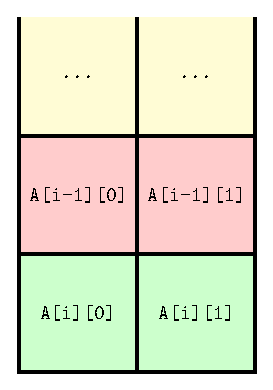
\includegraphics[height=0.3\textheight]{drawing-1/drawing-figure2.eps} }}%
    \qquad
    \subfloat[ ]{{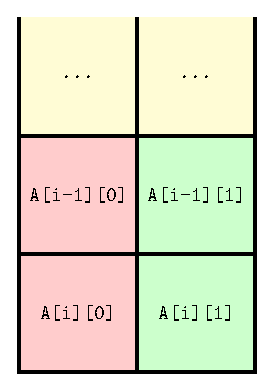
\includegraphics[height=0.3\textheight]{drawing-1/drawing-figure1.eps} }}%
    \qquad
    \subfloat[ ]{{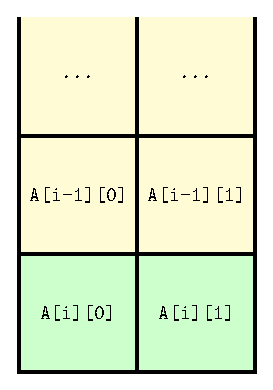
\includegraphics[height=0.3\textheight]{drawing-1/drawing-figure3.eps} }}%
    \qquad
\end{figure}

\item Если в решении используется конфигурация b, её можно заменить на a. Значит, можно считать, что мы всегда в 3 случае последний ряд заполняем одной костью, откуда имеем:
\[
\text{\texttt{dp[3][i][j]} = $\max\limits_{0 \leqslant k \leqslant 3}$ \texttt{dp[k][i-1][j-1]}+$\sum\limits_{0 \leqslant k \leqslant 1}$ \texttt{A[i][k]}} 
\]
\end{itemize}
\end{frame}








\begin{frame}
\frametitle{Задача №1}
\framesubtitle{Решение}
\fontsize{10pt}{7.2}\selectfont
\begin{itemize}
\item Если рассматривается случай, в котором только первая из двух клеток последнего ряда занята (случай 2), то есть два случая: когда клетка \texttt{[i-1][1]} покрыта и не покрыта костью:

\begin{figure}%
    \centering
    \subfloat[ ]{{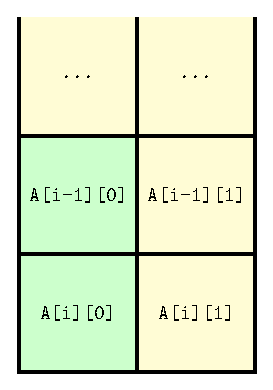
\includegraphics[height=0.3\textheight]{drawing-1/drawing-figure4.eps} }}%
    \qquad
    \subfloat[ ]{{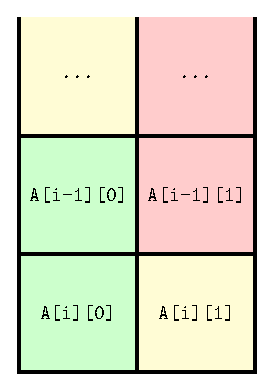
\includegraphics[height=0.3\textheight]{drawing-1/drawing-figure5.eps} }}%
    \qquad
\end{figure}

\item Отсюда имеем:
\begin{flalign*}
\text{\texttt{dp[1][i][j]}} =& \text{ $\max($\texttt{dp[0][i-1][j-1], dp[2][i-1][j-1]}$)$} +\\
+& \text{ \texttt{A[i][0]}}+\text{\texttt{A[i-1][0]}} 
\\\end{flalign*}
\item Аналогично выводится формула для \texttt{dp[2][i][j]}.
\end{itemize}
\end{frame}








\begin{frame}
\frametitle{Задача №1}
\framesubtitle{Решение}
\fontsize{10pt}{7.2}\selectfont
\begin{itemize}
\item Положим изначально 
\begin{itemize}
\item \texttt{dp[k][i][j]}$=-\infty$;
\item \texttt{dp[0][0][0] = 0};
\item \texttt{dp[3][0][1] = A[0][0] + A[0][1]};
\end{itemize}
\item С помощью вышеуказанных формул, можем тогда за $\mathcal O(NK)$ найти ответ.
\end{itemize}
\end{frame}








\begin{frame}
\frametitle{Задача №1}
\framesubtitle{Реализация}
\begin{itemize}
\item Чекер к данной задаче тривиален~--- считывая и проверяя на валидность решения жюри и участника, программа сверяет найденную сумму и возвращает вердикт~--- \texttt{OK}, если значение целевой функции совпало, \texttt{WA}, если жюри нашло ответ лучше и \texttt{FAIL} иначе.
\item Авторское решение реализует вышеописанную логику, работает за $\mathcal O(NK)$, написано на {C++}, что при ограничениях $N \times K \leqslant 2\cdot10^5$ работает на максимальном тесте не более чем за $0.2$  сек.
\end{itemize}
\end{frame}








\begin{frame}[fragile]
\frametitle{Задача №1}
\framesubtitle{Реализация}

\lstset{language=C++,
                basicstyle=\footnotesize \ttfamily,
                keywordstyle=\color{blue}\ttfamily,
                stringstyle=\color{red}\ttfamily,
                commentstyle=\color{green}\ttfamily,
                morecomment=[l][\color{magenta}]{\#}
}
Кусок кода с описанной выше логикой:
\begin{multicols}{2}
\begin{lstlisting}[basicstyle=\tiny]
for (int i = 0; i < 4; i++) {
    dp[i].resize(
        n, 
        vector<int>(k + 1, -INF)
    );
}

dp[0][0][0] = 0;
dp[3][0][1] = A[0][0] + A[0][1];

for (int i = 1; i < n; i++) {
    dp[0][i][0] = 0;
    for (int j = 1; j <= k; j++) {
        dp[0][i][j] = max(
            dp[0][i-1][j],
            dp[1][i-1][j],
            dp[2][i-1][j],
            dp[3][i-1][j]
        );

        dp[1][i][j] = max(
            dp[0][i-1][j-1],
            dp[2][i-1][j-1]
        ) + A[i][0] + A[i-1][0];

        dp[2][i][j] = max(
            dp[0][i-1][j-1],
            dp[1][i-1][j-1]
        ) + A[i][1] + A[i-1][1];

        dp[3][i][j] = max(
            dp[0][i-1][j-1],
            dp[1][i-1][j-1],
            dp[2][i-1][j-1],
            dp[3][i-1][j-1]
        ) + A[i][0] + A[i][1];
    }
}
int ans = max(
    dp[0][n-1][k],
    dp[1][n-1][k],
    dp[2][n-1][k],
    dp[3][n-1][k]
);
\end{lstlisting}

\end{multicols}
\end{frame}








\begin{frame}
\frametitle{Задачи №2-3}
\begin{itemize}
\item Задачи 2 и 3 имели \emph{открытые тесты}~--- они известны участнику и надо найти ответы к ним. Задачи носили оптимизационными задачами~--- точный ответ неизвестен и работа  оценивается в сравнении с лучшим известным решением.
\item Задача были дана на отборочном и финальном этапах олимпиады <<Московская олимпиада школьников>>\footnote{\url{http://mos-inf.olimpiada.ru/}}. Раунды проходил на платформе Яндекс.Контест.
\item Длительность отборочного этапа~--- несколько месяцев, финального этапа~--- 4 часа.
\end{itemize}
\end{frame}








\begin{frame}
\frametitle{Задача №2}
\framesubtitle{Условие}
\begin{itemize}
	\item Вариация известной NP-полной задачи SETCOV.
	\item Дано множество $A$ из $n$ элементов (все элементы -- числа от 1 до $n$). 
	\item Дано семейство $B$ из  $m$ подмножеств $A$. $i$-е подмножество содержит ровно $k_i$ элементов, равных $x_{i\, 1}, x_{i\, 2}, \ldots x_{i\, k_i}$. 
	\item Требуется выбрать какое-то подсемейство попарно непересекающихся множеств с максимальной мощностью объединения.
\end{itemize}
\end{frame}








\begin{frame}
\frametitle{Задача №2}
\framesubtitle{Решения}
\begin{itemize}
	\item Задачу можно детерминировано решить с помощью полного перебора за $\mathcal O \left(n\cdot2^m\right)$. 

	\item Если использовать \texttt{std::bitset} для хранения подмножеств, можно улучшить асимптотику до $\mathcal O \left(\frac{n2^m}{\omega}\right)$, где $\omega$~--- длина машинного слова.

	\item Если $m$ слишком велико, можно использовать рандомизированный алгоритм: выберем из данных $m$ множеств какое-то подсемейство размера $m_0 < m$ и решим задачу для этого 
	подсемейства за $\mathcal O \left(\frac{n2^{m_0}}{\omega}\right)$. Повторим операцию несколько раз и найдём среди найденных ответов лучший.
\end{itemize}
\end{frame}








\begin{frame}
\frametitle{Задача №2}
\framesubtitle{Решения}
\begin{itemize}
	\item Задачу можно решать как задачу оптимизации с помощью известных методов решения задачи оптимизации.
	\item Простейший вариант: поддерживать найденный ответ (подсемейство) и среди невключённых в него подмножеств пытаться включить какое-то множество, например, случайное или то, которое даёт наибольший прирост в значении целевой функции.
	\item Можно использовать \emph{метод имитации отжига} (simulated annealing), где модификации состояния~--- это включения и исключения каких-то подсемейств из ответа.
\end{itemize}
\end{frame}








\begin{frame}
\frametitle{Задача №2}
\framesubtitle{Решения}
\begin{itemize}
	\item Построим ориентированный граф, где вершины~--- это всевозможные подмножества множества $A$. Тогда проведём ребро из вершины $U \subset A$ в вершину $V \subset A$ тогда и только тогда, когда существует множество $C \subset B$, такое, что $U \sqcup C = V$.

	\item Путь из вершины $\varnothing$ в вершину $V$ говорит о том, что множество $V$ можно набрать подмножествами из $B$.

	\item Построим граф и найдём максимальную достижимую вершину с помощью алгоритма обхода в глубину за $\mathcal O\left(\frac{nm\cdot2^n}{\omega}\right)$
\end{itemize}
\end{frame}








\begin{frame}
\frametitle{Задача №2}
\framesubtitle{Реализация}
\begin{itemize}

\item Было сгенерировано $20$ тестов со следующими значениями $n$ и $m$:
\begin{xltabular}{\linewidth}{|l|l|l||l|l|l|}
\hline
\textbf{№} & \textbf{n}&  \textbf{m}& \textbf{№}&\textbf{n}&\textbf{m} \\\hline
1 & 5&  5 & 11 & 20 & 100 \\\hline
2 & 10 & 10 & 12 & 24 & 100 \\\hline
3 & 20 & 15 & 13 & 10000 & 10 \\\hline
4 & 100 & 20 & 14 & 10000 & 11 \\\hline
5 & 100 & 20 & 15 & 1000 & 30 \\\hline
6 & 100 & 20 & 16 & 1000 & 60 \\\hline
7 & 20 & 20 & 17 & 1000 & 60 \\\hline
8 & 20 & 40 & 18 & 9999 & 100 \\\hline
9 & 20 & 60 & 19 & 10000 & 100 \\\hline
10 & 20 & 100 & 20 & 10000 & 100 \\\hline
\end{xltabular}

% \item Чекер к данной задаче тривиален~--- считывая и проверяя на валидность решения жюри и участника, программа сверяет найденную сумму и возвращает вердикт~--- \texttt{OK}, если значение целевой функции совпало, \texttt{WA}, если жюри нашло ответ лучше и \texttt{FAIL} иначе.
% \item Авторское решение реализует вышеописанную логику, работает за $\mathcal O(NK)$, написано на {C++}, что при ограничениях $N \times K \leqslant 2\cdot10^5$ работает на максимальном тесте не более чем за $0.2$  сек.
\end{itemize}
\end{frame}








\begin{frame}
\frametitle{Задача №2}
\framesubtitle{Реализация}
% \fontsize{11pt}{7.2}\selectfont
\begin{itemize}
\item В качестве оценки решения участника была выбрана формула $$5 \times\left(\frac{\text {ParticipantSolution}}{\text {BestSolution}}\right)^{3}$$где $\text{ParticipantSolution}$~--- значение целевой функции в решении участника, а $\text{BestSolution}$~--- лучший найденный ответ.

\item Чекер к данной задаче тривиален~--- считывая и проверяя на валидность решения жюри и участника, программа сверяет найденные ответы и возвращает балл по формуле выше.

\item Главное авторское решение реализует алгоритмы, описанные в разделе с решениями.

\end{itemize}
\end{frame}








\begin{frame}
\frametitle{Задача №3}
\framesubtitle{Условие}
\begin{itemize}
\item Сокобан~--- логическая игра-головоломка, в которой игрок передвигает ящики по лабиринту, показанному в виде плана, с целью поставить все ящики на заданные конечные позиции. 
\item Сокобан может двигаться вверх, вниз, влево и вправо. Он не может проходить сквозь стены или ящики. Он может толкать только одну коробку за раз.
\item Известна конфигурация лабиринта~--- поля $n\times m$, состоящая из пустых клеток или стен. Также известна начальная позиция каждого из ящиков, конечные позиции, куда надо поставить ящики и начальное положение Сокобана.
\item Необходимо найти кратчайший способ решить головоломку~--- найти наиболее короткий (по числу действий) способ поставить все ящики на позиции.
\end{itemize}
\end{frame}








\begin{frame}
\frametitle{Задача №3}
\framesubtitle{Условие}
Пример головоломки и её решения:
\begin{figure}[ht]
\begin{center}
   \makebox[\textwidth][c]{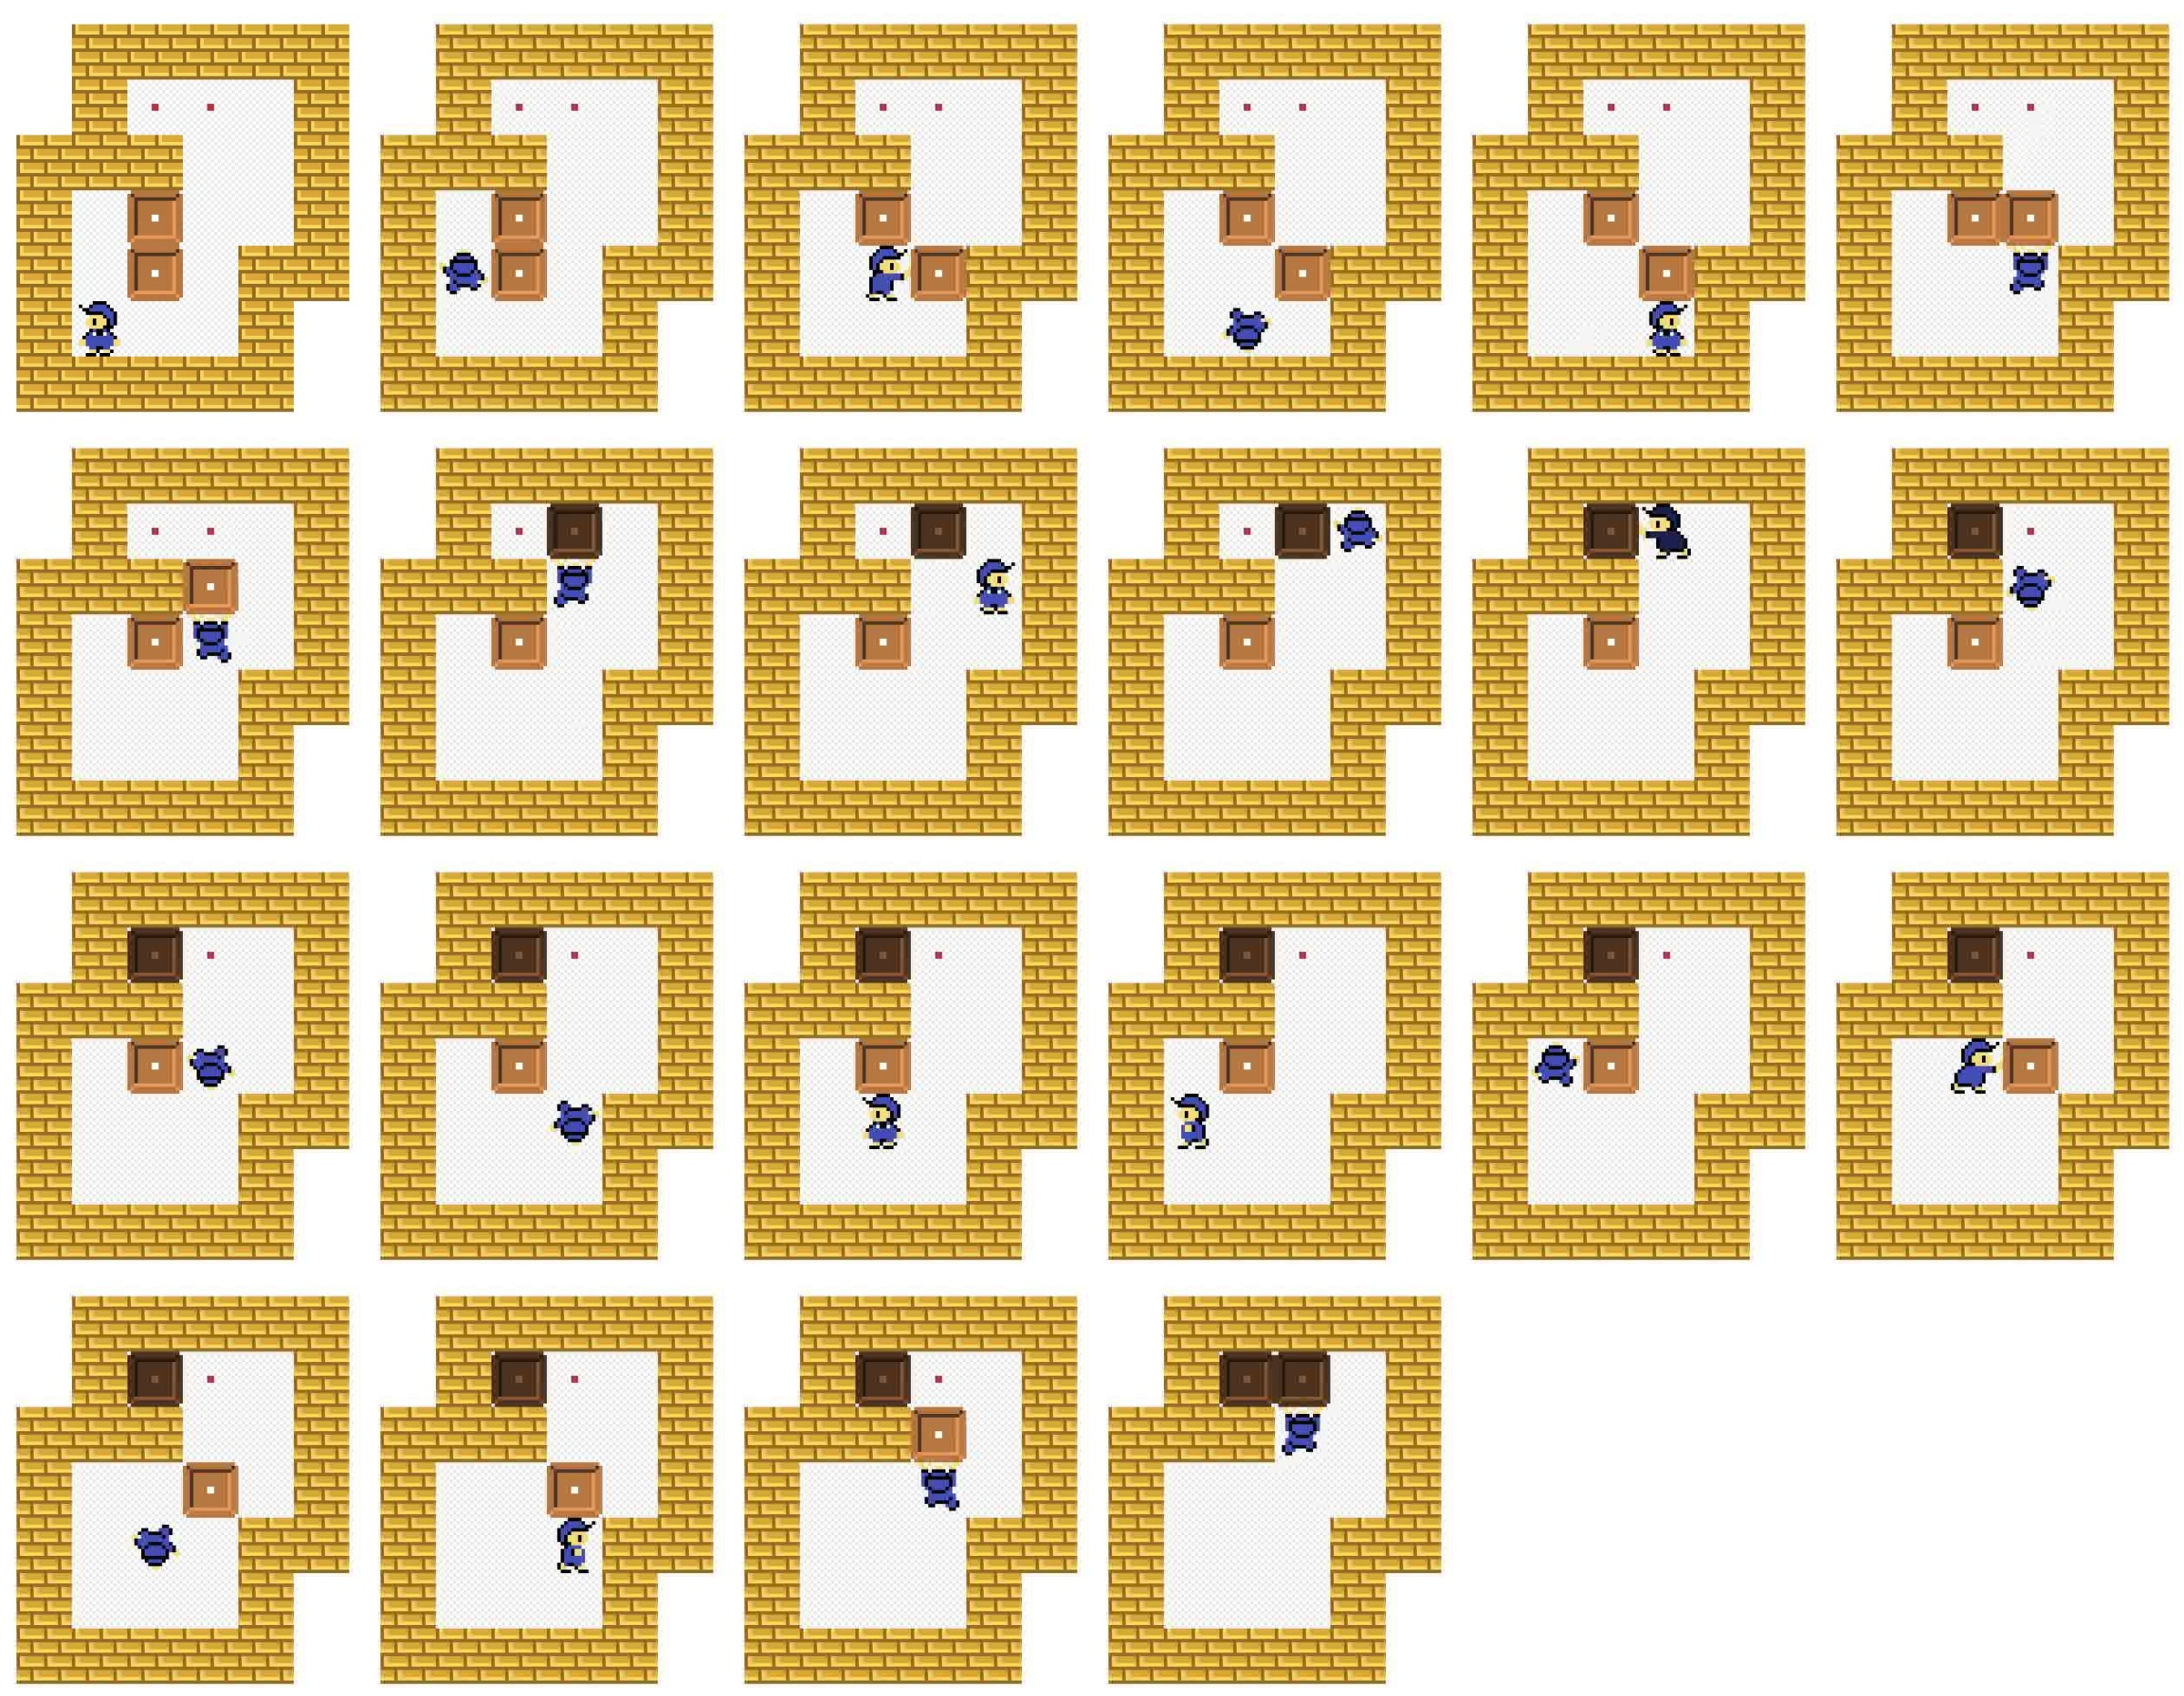
\includegraphics[width=0.8\textwidth]{../mosinf-sokoban/statement/example-sokoban.jpg}}
\end{center}
\end{figure}
\end{frame}








\begin{frame}
\frametitle{Задача №3}
\framesubtitle{Решение}
\begin{itemize}
\item Рассмотрим граф, состоящий из всевозможных конфигураций (конфигурация -- это совокупность положений ящика и сокобана), где ребро ставится из вершины $A$ в вершину $B$ тогда и только тогда, когда из конфигурации $A$ при шаге сокобана в одном из направлений, лабиринт перейдёт в состояние B. 
\item Обозначим за $S$ стартовое состояние, а за $\left\{T_i\right\}$~--- все конечные состояния. Проведём рёбра из $\left\{T_i\right\}$ в фиктивную вершину $T$.
\item Задача свелась к задаче поиска кратчайшего пути из $S$ в $T$.
\end{itemize}
\end{frame}








\begin{frame}
\frametitle{Задача №3}
\framesubtitle{Решение}
\begin{itemize}
\item В качестве базового решения можно рассмотреть \emph{BFS} (поиск в ширину). Его решение оправдано, так как хотя граф и может быть очень большим, ответ практически всегда достаточно мал.
\item Можно оптимизировать $BFS$ таким образом, чтобы не рассматривать гарантированно тупиковые конфигурации, например, те, в которых ящик стоит в углу~--- оттуда достать его будет невозможно:
    \begin{figure}
    \centering
    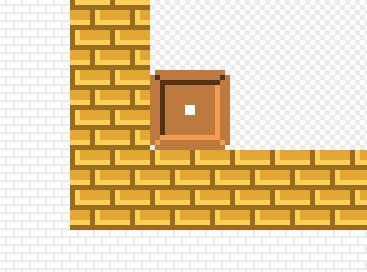
\includegraphics[width=0.3\textwidth]{photo_2020-06-29_01-28-58.jpg}
    \end{figure}
\end{itemize}
\end{frame}








\begin{frame}
\frametitle{Задача №3}
\framesubtitle{Решение}
\begin{itemize}
\item Можно оптимизировать BFS, с помощью метода \emph{meet-in-the-middle}:
\begin{itemize}
\item Запустим два алгоритма BFS: в начальном графе из стартовой вершины и в транспонированном графе из конечной вершины
\item Будем поочерёдно запускать по фазе BFS ($d$-я фаза находит все вершины, расстояние до которых равно $d$) в одном алгоритме и другом.
\item Если они оба найдут кратчайший путь до какой-то вершины $v$, то будет найден кратчайший путь до вершины $v$ из $S$ и кратчайший путь до $T$ из вершины $v$
\item Можно показать, что объединение этих путей будет искомым кратчайшим путём.
\end{itemize}
\end{itemize}
\end{frame}








\begin{frame}
\frametitle{Задача №3}
\framesubtitle{Реализация}
\begin{itemize}
\item Было решено, что решения, использующие простой BFS будут набирать $30\%$ баллов, а двунаправленный BFS~--- все баллы.
\item Для генерации тестов были выбраны уже известные головоломки сокобан, порядка 3 тысяч
\item Авторское решение было протестировано на каждом из них, замеряя время работы обычного BFS, двухстороннего BFS, а также объём потребляемой памяти.
\item В первую группу (15 тестов) были отобраны тесты, суммарное время работы на которых обычного BFS не превосходило 2 минут. Во вторую группу (25 тестов) были отобраны тесты, суммарное время работы полного решения на которых не превосходило 8 минут, и при этом решение с использование обычного BFS не работало в связи с ограничениями по памяти или времени.
\end{itemize}
\end{frame}








\begin{frame}
\frametitle{Задача №3}
\framesubtitle{Реализация}
\begin{itemize}
\item В качестве оценки решения участника была выбрана формула $$2 \times\left(\frac{\text {BestSolution}}{\text {ParticipantSolution}}\right)^{4}$$где $\text{ParticipantSolution}$~--- длина пути в решении участника, а $\text{BestSolution}$~--- лучший найденный путь.
\item Чекер к данной задаче тривиален~--- считывая и проверяя на валидность решения жюри и участника (эмулируя работу головоломки), программа сверяет найденные ответы и возвращает балл по формуле выше.
\item Главное авторское решение реализует алгоритм, описанные в разделе с решениями.
\end{itemize}
\end{frame}








\begin{frame}
\frametitle{Задача №3}
\framesubtitle{Реализация}
\begin{itemize}
\item Главное решение не хранит граф явно, а генерирует все рёбра только тогда, когда обрабатывает очередную вершину
\item Вершины хранятся как массивы чисел, где первое число~--- положение сокобана, а остальные числа~--- сортированные положения коробок.
\item Положение~--- число от 0 до 255 (предполагается, что все поля достаточно маленькие). Для хранения массивов положений используется \texttt{std::pair<long long, long long>} (в качестве массива из 16 байт)
\item Это сделано для оптимизации времени и памяти, используемых программой.
\end{itemize}
\end{frame}








\begin{frame}
\frametitle{Тестирование проекта}
Перед проведением олимпиад проходит \emph{ <<прорешивание>> } задач заинтересованными людьми~--- организатором олимпиады, членами методической комиссии, студентами. Их отзывы по подготовленным задачам были приняты во внимание, недочёты исправлены.
\end{frame}








\begin{frame}
\fontsize{11pt}{7.2}\selectfont
\frametitle{Основные результаты работы}
\begin{enumerate}
\item Были подготовлены 3 задачи, используя которые были проведены туры перечневых олимпиад по программированию.
\item Первая задача была предложена более чем 1000 участникам, вторая~--- более чем 2500, третья~--- более чем 300.
\item Подготовленные пакеты функционировали как и предполагалось, значимых неполадок в течении тура не наблюдалось.
\item По 3 задаче 45 участников отправляли решения, по 2 задаче было предпринято свыше 1900 посылок.
\item Большинство задач оказались не слишком простыми и не слишком сложными~--- в их решении требовались знания, связанные со спортивным программированием, равно как и умение оптимально писать код. 
\end{enumerate}
\end{frame}


\begin{frame}
\frametitle{Направления дальнейшей работы}
Разработанные задачи нельзя назвать тупиковыми: так, каждую из них можно упростить или усложнить и переиспользовать в дальнейшем.
\begin{enumerate}
\item Например, если рассмотреть 1 задачу но уже на полоске $N \times M$ вместо $N \times 2$, концептуально решение не поменяется, но аналогичное решение, работая за $\mathcal O(KN2^M)$, будет гораздо сложнее в реализации.
\item Во 2 и 3 задачах можно уменьшать и увеличивать ограничения на входные данные, требуя тем самым более сложные или оптимальные решения.
\end{enumerate}

\end{frame}








\begin{frame}[typeset second]
\begin{center}
{\LARGE Спасибо за внимание.} \\
\bigskip
Деб Натх Максим \\\smallskip \scriptsize \url{mdebnatkh@edu.hse.ru}\\\url{debnatkh@gmail.com}

\bigskip
\scriptsize{Москва, 2020}
    \end{center}
\end{frame}








\end{document}


